\documentclass{article}
\usepackage{graphicx} % Required for inserting images
\usepackage[a4paper, total={6in, 8in}, margin=1in]{geometry}
\usepackage{listings}
\usepackage{hyperref}
\usepackage{amsmath}
\usepackage{amssymb}
\usepackage{authblk}
\usepackage{float}
\usepackage{parskip}
\usepackage{minted}
\usepackage{fontawesome}
\usemintedstyle{vs}
\newcommand{\ts}{\textsuperscript}



\begin{document}

\begin{titlepage}
    \centering
    \vspace*{1cm}
    
    % Insert image (adjust width as needed)
    
    
    
    
    % Title
    {\Huge\bfseries INF219 – COWI Research \par}
    
    
    \vspace{1.5cm}
    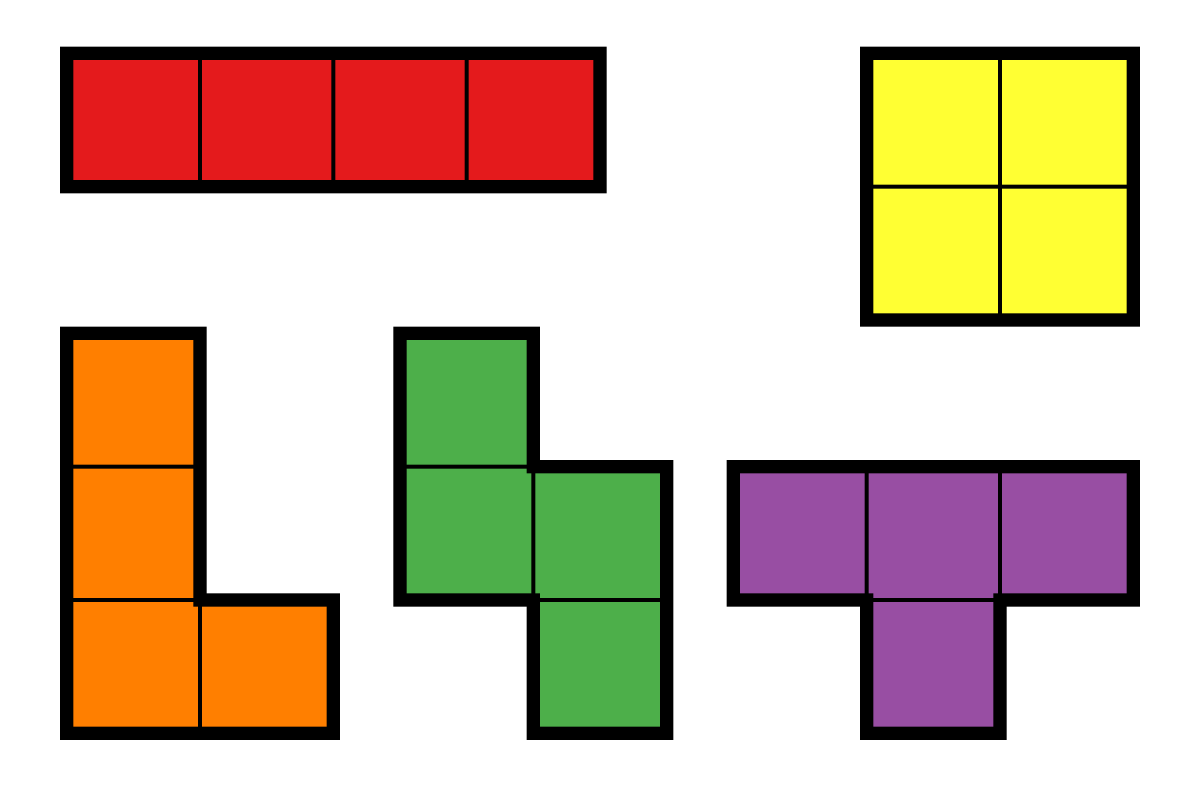
\includegraphics[width=0.5\textwidth]{tetris.png} % replace with your image file name
    \vspace{1cm}
    % Authors

    {\large Jakob Sverre Alexandersen \\
    Thone Anlaug Stordal Støa \\
    Hanna Søndenaa Rasmussen \\
    Håvard Kattem Lunde \\
    Hermann Holstad Walaunet \par}
    
    
    \vfill
    
    % Footer
    {\large April 2025 \par}
    
    \vspace{1cm}
    \href{https://github.com/alexandersen01/COWI-research}{\faicon{github} GitHub Repository}
\end{titlepage}


\newpage

\tableofcontents

\newpage

\section{Summary}

Click me: \href{https://github.com/alexandersen01/COWI-research}{\faicon{github}} for the full repo

\hrulefill{}

This project considers techniques for placing light fixtures in any given room, 
minimizing the amount of lights used whilst still being compliant with regulatory
and aesthetic requirements.

There are many different approaches to such a challenge. For instance, COWI presented
a genetic algorithm/reinforcement learning ML-based solution. Their approach 
entailed maximizing coverage area while maintaining a pattern by penalizing variations
in x/y coordinates. 

We chose to take a different approach, using Linear Programming instead. The main reason
behind this choice is the guaranteed optimality involved in such a solution.
Using a solver, we are able to find the single most mathematically optimal solution 
that satisfies all constraints, given that a solution exists.

In addition to the optimality, we are also presented with several other advantages 
using the LP approach. The deterministic nature of our solution ensures that given 
the same inputs and constraints, we always get identical, reproducible 
results — eliminating the randomness inherent in genetic algorithms. This 
consistency is particularly valuable in professional settings where repeatability 
is essential.

Our LP formulation also offers greater transparency and explainability, making it 
clear exactly what we're optimizing for and what constraints we're satisfying. 
For typical room dimensions, the LP solver finds optimal solutions relatively quickly, 
without requiring the multiple generations of evolution that genetic algorithms need. 
This efficiency translates to faster design iterations and project delivery.
The precise constraint handling in our approach allows for explicit modeling of 
critical requirements like minimum light levels and fixture spacing. Rather than 
approximating these through penalty functions as in the genetic algorithm approach, 
we incorporate them directly into the mathematical model.
Finally, our solution offers straightforward adaptability to changing requirements. 
The LP model parameters can be easily adjusted to meet different regulatory 
standards or design preferences without needing to retrain an entire ML model. 
While the ML-based approach might offer advantages in terms of continuous 
learning from historical data, our LP solution provides immediate, verifiable 
results with mathematical guarantees—a critical factor when dealing with 
safety-related regulatory compliance in building design. This becomes a bigger deal
if we choose to also incorporate positioning of a sprinkler system.

\newpage

\section{Motivation and Introduction (Thone)}

\newpage

\section{Mathematics (jakob se over)}

In this section, we will discuss the mathematical model behind the program.

\subsection{Sets and Indices}
\begin{align}
    G &= \{(x, y) \mid (x, y) \in \mathbb{R}^2\} \quad \text{(Grid points for potential circle placement)}\\
    A &= \{(x, y) \mid (x, y) \in \mathbb{R}^2\} \quad \text{(Area cells for measuring coverage)}
\end{align}

\subsection{Decision Variables}
\begin{align}
    z_{x, y} &\in \{0, 1\} \quad \forall (x, y) \in G \quad \text{(Binary variable for circle placement)}\\
    c_{x, y} &\geq 0 \quad \forall (x, y) \in A \quad \text{(Continuous variable for cell light level)}
\end{align}

\subsection{Parameters}
\begin{align}
    \alpha_{(x_g, y_g), (x_a, y_a)} &\geq 0 \quad \text{(Coverage value from grid point to area cell)}\\
    L_{\min} &\geq 0 \quad \text{(Minimum required average light level)}\\
    S_{\min} &\geq 0 \quad \text{(Minimum required spacing between circles)}\\
    A_g &\subset A \quad \text{(Set of area cells within grid cell $g \in G$)}
\end{align}

\subsection{Objective Function}
\begin{align}
    \min \sum_{(x, y) \in G} z_{x, y} \quad \text{(Minimize total number of circles)}
\end{align}

\subsection{Constraints}
\begin{align}
    c_{x_a, y_a} &= \sum_{(x_g, y_g) \in G} \alpha_{(x_g, y_g), (x_a, y_a)} \cdot z_{x_g, y_g} \quad \forall (x_a, y_a) \in A\\
    \sum_{(x_a, y_a) \in A_g} c_{x_a, y_a} &\geq L_{\min} \cdot |A_g| \quad \forall g \in G \text{ where } |A_g| > 0\\
    z_{x_1, y_1} + z_{x_2, y_2} &\leq 1 \quad \forall (x_1,y_1),(x_2,y_2) \in G \text{ where } \max\left(\frac{|x_1-x_2|}{\text{grid\_size}}, \frac{|y_1-y_2|}{\text{grid\_size}}\right) \leq S_{\min}
\end{align}

\subsection{Constraints explainations}

\begin{enumerate}
    \setcounter{enumi}{9}
    \item Defines how the light level for each area cell is calculated
    \item Ensures that each grid cell receives adequate light
    \item Prevents lights from being placed too close to each other
    \item TODO add neigh constraint 
\end{enumerate}

\newpage

\section{Execution}

In this section we will shine some light on how we chose to solve the main problem – finding the optimal solution via a generic algorithm 
for placing light fixtures in any room of any size.

\subsection{Method (jakob)}

As previously mentioned, a genetic algorithm/RL approach was presented to us. Although this can be a good solution in some cases, we found out that
this method does not provide heuristics that are sufficiently effective or efficient for approximating the optimal solution.

Our approach to optimizing light fixture placement employs linear programming (LP), a powerful mathematical optimization technique that allows us to 
find the exact minimum number of fixtures required while satisfying all regulatory and aesthetic constraints.

The problem is formulated as a binary integer linear program where each potential fixture location is represented by a binary decision 
variable. The objective function minimizes the total number of fixtures, subject to a set of constraints that ensure adequate light coverage 
and appropriate spacing between fixtures. 

The room is first resized into a smaller polygon. The reason for this is so that we can avoid considering not placing lights near the walls. 
This is a relatively easy and efficient way of minimizing computational cost as we don't need to define this in the constraints. Next up, we 
discretize the room into a grid, where each grid point represents a potential fixture location. A finer grid of area cells is then used to evaluate
light coverage with precision. For each area cell, we calculate the light contribution from all potential fixture locations, creating a coverage
model that accounts for light falloff with distance. 

Two primary constraint types govern our solution; coverage constraints ensure that each area maintains at least the minimum required light level 
(lux) specified by regulations, while spacing constraints enforce a minimum distance between fixtures to create aesthetically pleasing and 
practically functional layouts. 

Unlike heuristic approaches such as genetic algorithms that approximate solutions, our LP formulation guarantees finding the mathematically optimal 
solution whenever one exists. This mathematical certainty is particularly valuable in contexts where regulatory compliance must be definitively
demonstrated. 

The model's flexibility allows for straightforward parameter adjustments to accomodate different regulatory standards or design preferences. 
By simply modifying the minimum lux parameter or the fixture spacing requirement, the model can be adapted to various building types and usage 
scenarios without requiring findamental changes to the underlying optimization approach.

Implementation is achieved using the PuLP library in Python, which interfaces with powerful LP solvers capable of handling the binary 
integer programming challenges in the problem space.

\subsection{What we tried: (hanna) (talk about our shortcomings)}

\newpage

\section{Experiments (TBD)}
\subsection{Light distribution plot}
\subsection{Small room}
\subsection{Large room}
\subsection{Runtime Discussion}



\newpage

\section{Discussion (Håvard)}

\subsection{Potential Improvements}
\subsubsection{Caching}

\newpage

\section{Conclusion (Hermann)}

In this project, we have explored two approaches to lighting optimization using the PuLP library, a mixed-integer programming solver.
The first model uses a simple mathematical grid patterning approach that places lights based on fixed spacing rules, independent of actual lighting values.
This results in visually good, regular arrangements, but lacks adaptability to lighting requirements.

The second model is a constraint-based optimization solution that mathematically ensures compliance with lighting thresholds,
fixture spacing, and other constraints. This model provides precise results and guarantees that the lighting meets the minimum lux requirement
throughout the room. However, the output can sometimes appear less pleasing, especially in irregular spaces, as the focus is purely on optimization rather than visual symmetry.

Through our experiments, we observed that the optimization model performs particularly well when the required lighting level is higher,
such as 300 lux or more. In such cases, the denser fixture placement leaves more room for the solver to balance aesthetics and coverage.
Conversely, at low lux requirements, the model tends to use fewer lights and may produce more irregular patterns.

The project was carried out through structured collaboration, with group meetings and division of tasks ensuring even distribution of work 
and collective problem-solving. Together, we have demonstrated how linear programming can be a powerful tool
in practical engineering contexts, offering both adaptability and mathematical rigor.


\end{document}